\documentclass{article}
\usepackage[utf8]{inputenc}
\usepackage{url}
\usepackage{authblk}

\title{Three Algorithms for Merging Navigable Graphs}
\author[1]{Alexander Ponomarenko}
\date{}


% \affil[2]{YugaByte LLC}
\affil[1]{HSE Univerity}

\usepackage{natbib}
\usepackage{graphicx}
\usepackage{subcaption}
\usepackage{algorithm}
\usepackage{algorithmicx}
\usepackage[noend]{algpseudocode}
\usepackage{amsmath}
\DeclareMathOperator*{\argminA}{arg\,min} % Jan Hlavacek
\DeclareMathOperator*{\argminB}{argmin}   % Jan Hlavacek
\usepackage{amsfonts}
\usepackage{amssymb}
\usepackage{nameref}
\begin{document}

\maketitle

\section{Introduction}
Navigable small-world graphs have emerged as a cornerstone for efficient approximate nearest neighbor (ANN) search in high-dimensional spaces. This problem is crucial in fields such as recommendation systems, image retrieval, and natural language processing. Algorithms like Hierarchical Navigable Small World (HNSW) \cite{hnsw} and its predecessor Navigable Small World (NSW) \cite{nsw2011,nsw2012,nsw2014} provide robust and scalable frameworks for organizing data into graph structures that support fast similarity searches.

One key limitation of these methods is the absence of a natural mechanism for node deletion, which is essential as datasets evolve and obsolete items accumulate. This necessitates merging and compacting graphs to maintain efficiency and accuracy in the search index over time.

While HNSW supports dynamic insertions, it lacks native support for deletions. As a result, merging becomes a form of "compaction," where graphs from two or more sources are combined, and nodes marked for deletion are omitted. This not only improves space efficiency but also enhances search quality by reducing noise from irrelevant entries.

In this work, we propose three novel algorithms—\textbf{Naive Merge}, \textbf{Merge1}, and \textbf{Merge2}—for efficiently merging navigable graphs. While our methods primarily target HNSW, they are generalizable to other graph-based data structures such as NSW \cite{nsw2011} and NSG \cite{NSG}. These algorithms preserve graph navigability and ensure that deleted nodes are excluded from the merged result, maintaining the structural integrity necessary for fast ANN search.

\section{Search}

We begin by describing basic search operations over a single graph.

\begin{algorithm}
\caption{\textsc{LocalSearch}($G, q, C, k, L$)}\label{alg:local_search}
\textbf{Input:} Graph $G = (V, E)$, query $q \in \mathbb{R}^d$, initial candidate set $C \subset V$, $k \in \mathbb{N}$, $L \in \mathbb{N}$ \\
\textbf{Output:} Approximate $k$-nearest neighbors $V^* \subset V$
\begin{algorithmic}[1]
% \State $C \gets \textsc{InitializeCandidates}()$
\While{True}
    \State $u \gets$ nearest unvisited point to $q$ in $C$
    \State $U \gets \{v \mid (u, v) \in E\}$
    \For{$v \in U$}
        \If{$v$ is unvisited}
            \State $C \gets C \cup \{v\}$
        \EndIf
    \EndFor
    \If{$|C| > L$}
        \State $C \gets$ top $L$ nearest points to $q$ in $C$
    \EndIf
    \If{no updates to $C$}
        \State \textbf{break}
    \EndIf
\EndWhile
\State \Return top-$k$ nearest points to $q$ in $C$
\end{algorithmic}
\end{algorithm}

The parameter $L$ controls the breadth of the search and helps avoid getting trapped in local minima. In the HNSW paper, it is referred to as the \textbf{ef} (expansion factor) parameter.

\begin{algorithm}
\caption{\textsc{HNSW-Search}($\mathcal{H}, q, v_0, k, L, \ell$)}\label{alg:hnsw_search}
\textbf{Input:} HNSW graph $\mathcal{H} = (G_i)_{i=0}^{l_{\max}}$, query $q \in \mathbb{R}^d$, starting vertex $v_0 \in V$, $k, L \in \mathbb{N}$, search layer $\ell$ \\
\textbf{Output:} Approximate $k$-nearest neighbors $V^* \subset V$
\begin{algorithmic}[1]
\State $v^* \gets v_0$ 
\For{$i = l_{\max} \textbf{ down to } \ell$}
    \State $v^* \gets \textsc{LocalSearch}(G=G_i, q=q, C=\{v^*\}, k=1, L=L)$
\EndFor
\State \Return \textsc{LocalSearch}$(G_\ell, q, \{v^*\}, k, L)$
\end{algorithmic}
\end{algorithm}

\section{Neighborhood Construction Strategies}

Various strategies exist for selecting a node's neighborhood. Our merging algorithms are agnostic to the specific neighborhood construction method, which can be provided as a parameter.

\begin{algorithm}
\caption{\textsc{KNN-Neighborhood-Construction}($v^*, C, k$)}\label{alg:knntrategy}
\textbf{Input:} Vertex $v^*$, candidate set $C$, number of neighbors $k$ \\
\textbf{Output:} Set $C'$ of $k$ closest neighbors
\begin{algorithmic}[1]
\State $C' \gets$ $k$-nearest neighbors of $v^*$ in $C$
\State \Return $C'$
\end{algorithmic}
\end{algorithm}

\begin{algorithm}
\caption{\textsc{RNG-Neighborhood-Construction}($v^*, C, m$)}\label{alg:rngstrategy}
\textbf{Input:} Vertex $v^*$, candidate set $C$, maximum neighborhood size $m$ \\
\textbf{Output:} Filtered neighbor set $C'$
\begin{algorithmic}[1]
\State Sort $C$ in ascending order by distance to $v^*$
\State $C' \gets \emptyset$
\For{$v \in C$}
    \State $f \gets$ true
    \For{$w \in C'$}
        \If{$\rho(v^*, v) \geq \rho(v, w)$}
            \State $f \gets$ false
            \State \textbf{break}
        \EndIf
    \EndFor
    \If{$f$}
        \State $C' \gets C' \cup \{v\}$
    \EndIf
    \If{$|C'| \geq m$}
        \State \textbf{break}
    \EndIf
\EndFor
\State \Return $C'$
\end{algorithmic}
\end{algorithm}

\section{Merge Algorithms}


%We provide 3 merge algorithms: "Naive Merge", "Merge1", and "Merge2". We also refer to these algorithm as layer-merge algorithms. "Naive Merge" is a straight forward method, while "Merge1" and "Merge2" are more advanced. Together, these two algorithms constitute the main contribution of the work. The HNSW structure is a sequence of graphs, called layers. We start from description of a general algorithm for merging multi layers structure.
We now present three algorithms for merging HNSW graphs: \textsc{Merge-Naive}, \textsc{Merge1}, and \textsc{Merge2}. These algorithms operate layer by layer. We first describe the general procedure for merging the multi-layer HNSW structure, followed by the specific logic for merging a single layer (\textit{layer-merge algorithms}).

\subsection{HNSW General Merge Framework}

The \textsc{HNSW-General-Merge} algorithm (Algorithm~\ref{alg:general_merge}) provides a framework for merging two HNSW structures, $\mathcal{H}_a$ and $\mathcal{H}_b$. It iterates through each layer level and applies a chosen layer-merge algorithm (\textsc{Merge-Naive}, \textsc{Merge1}, or \textsc{Merge2}) to combine the corresponding layers $G^a_i$ and $G^b_i$. The layer-merge algorithms require access to the full HNSW structures $\mathcal{H}_a, \mathcal{H}_b$ to perform efficient searches (using \textsc{HNSW-Search} or \textsc{LocalSearch}) down to the target layer $\ell=i$.

Let $l_{\max}^a$ and $l_{\max}^b$ be the maximum layer indices for $\mathcal{H}_a$ and $\mathcal{H}_b$, respectively. The merged graph $\mathcal{H}_c$ will have $l_{\max}^c = \max(l_{\max}^a, l_{\max}^b)$ layers.

\begin{algorithm}
\caption{\textsc{HNSW-General-Merge}($\mathcal{H}_a, \mathcal{H}_b, \text{LayerMergeAlgo}, \text{params}$)}\label{alg:general_merge}
\textbf{Input:} HNSW graphs $\mathcal{H}_a$, $\mathcal{H}_b $. Chosen layer merge algorithm $\text{LayerMergeAlgo}$ (e.g., \textsc{Merge-Naive}). Algorithm-specific parameters $\text{params}$. \\
\textbf{Output:} Merged HNSW graph $\mathcal{H}_c = (G^c_i)_{i=0}^{l_{\max}^c}$
\begin{algorithmic}[1]
\State $l_{\max}^a \gets \mathcal{H}_a.\text{getMaxLayerNumber()}$
\State $l_{\max}^b \gets \mathcal{H}_b.\text{getMaxLayerNumber()}$
\State $l_{\max}^c \gets \max(l_{\max}^a, l_{\max}^b)$
\For{$i = 0 \textbf{ to } l_{\max}^c$} \Comment{Merge each layer}    
    \State $G^c_i \gets \text{LayerMergeAlgo}(\mathcal{H}_a, \mathcal{H}_b, \ell=i, \text{params})$ \Comment{Calls e.g., Merge-Naive}
\EndFor
\State $\mathcal{H}_c \gets (G^c_i)_{i=0}^{l_{\max}^c}$ % Construction is implicit in the loop

\State \Return $\mathcal{H}_c$
\end{algorithmic}
\end{algorithm}

Note that the merging of different layers (iterations of the loop in Algorithm~\ref{alg:general_merge}) is independent and can potentially be parallelized.



%\subsection{Naive Merge}
%The Naive Merge algorithm \ref{alg:merge_naive} surprisingly is very simple. It takes one vertex $v^*$ by one from the graph $G^a$. Then algorithm prepares the candidate set $\mathcal{C}$ for a new neighborhood (lines 6,7). It uses \textsc{HNSW-Search} to get $m$-closest vertices to $v^*$ in the graph $G^b$, and combines with an old neighborhood of the vertex $v^*$. After that in the line 8 the candidate set $\mathcal{C}$ is passed into the neighborhood construction function, which selects the vertices for the new merged neighborhood for $v^*$.
%Lines 9-12 contains the same logic for the forming new neighborhoods of graph $G^b$

\subsection{Naive Merge}
The \textsc{Merge-Naive} algorithm (Algorithm~\ref{alg:merge_naive}) provides a straightforward method for merging a single layer $\ell$. For each vertex $v^*$ originating from graph $G^a_\ell$, it searches for its potential neighbors in graph $G^b_\ell$ using the full \textsc{HNSW-Search} procedure down to layer $\ell$. These candidates are combined with the original neighbors of $v^*$ in $G^a_\ell$. The final neighborhood for $v^*$ in the merged graph $G^c_\ell$ is selected from this combined set using the chosen \textsc{NeighborhoodConstruction} strategy. The process is repeated for vertices originating from $G^b_\ell$.






\begin{algorithm}
\caption{\textsc{Merge-Naive}($\mathcal{H}_a, \mathcal{H}_b, \ell, \text{NeighborhoodConstruction}, m, \text{search\_ef}, v_{entry}$)}\label{alg:merge_naive}
\textbf{Input:} HNSW graphs $\mathcal{H}_a$, $\mathcal{H}_b$; target layer $\ell$; Neighborhood construction function \textsc{NeighborhoodConstruction}; target neighborhood size $m$; search parameter $\text{search\_ef}$; entry point $v_{entry}$ (e.g., from $\mathcal{H}_a$ or $\mathcal{H}_b$) \\
\textbf{Output:} Merged graph $G^c$
\begin{algorithmic}[1]
\State $G^a \gets \mathcal{H}_a\text{.GetLayer}(\ell) $; $G^b \gets\mathcal{H}_a\text{.GetLayer}(\ell)$ 
\State $V^a \gets \text{vertices}(G^a)$; $V^b \gets \text{vertices}(G^b)$
\State $E^a \gets \text{edges}(G^a)$; $E^b \gets \text{edges}(G^b)$
\State $V^c \gets V^a \cup V^b$; $E^c \gets \emptyset$ \Comment{Initialize vertices and edges for the merged graph}
% \State $m \gets \dots$ % Now passed as input parameter

\For{$v^* \in V^a$} \Comment{Process vertices from graph A}
    \State $\mathcal{C}^b \gets \textsc{HNSW-Search}(\mathcal{H}=\mathcal{H}_b, q=v^*, v_{entry}=v_{entry}^b, k=m, L=\text{search\_ef}, \ell=\ell)$ \Comment{Find candidates in B}
    \State $\mathcal{C} \gets \{v \mid (v^*, v) \in E^a \} \cup \mathcal{C}^b$  \Comment{Combine original neighbors and candidates from B}
    \State $E^c \gets E^c \cup \{(v^*, v) | v \in \textsc{neighborhood\_construction}(\mathcal{C}, v^*, m)\}$\Comment{Add new neighborhood to set of edges}
\EndFor

\For{$v^* \in V^b$} \Comment{Process vertices from graph B}
    \State $\mathcal{C}^a \gets \textsc{HNSW-Search}(\mathcal{H}=\mathcal{H}_a, q=v^*, v_{entry}=v_{entry}^a, k=m, L=\text{search\_ef}, \ell_{target}=\ell)$ \Comment{Find candidates in A}
    \State $\mathcal{C} \gets \{v \mid (v^*, v) \in E^b \} \cup \mathcal{C}^a$  \Comment{Combine original neighbors and candidates from A}
    \State $E^c \gets E^c \cup \{(v^*, v) | v \in \textsc{neighborhood\_construction}(\mathcal{C}, v^*, m)\}$\Comment{Add new neighborhood to set of edges}
\EndFor

\State \Return $G^c = (V^c, E^c)$
\end{algorithmic}
\end{algorithm}


This naive approach is simple but computationally intensive due to repeated \textsc{HNSW-Search} calls, each potentially traversing multiple layers from the top down.


\subsection{Merge1}
The most effort of \textsc{Merge-Naive} algorithm lies in the set of neighborhood candidates from the opposite graph utilising \textsc{HNSW-Search} procedure, that traverses layers graph from the top-level down to layer number $\ell$ every time. The number of computations can be reduced if we select the next vertex $v^*$ close to the previous one (line 15), instead of choosing it randomly. Thus, for new $v^*$ the neighborhood candidates will be  also close to the previous candidates set. To search this new neighborhood candidates we can use \textsc{LocalSearch} procedure, that traversing the same graph staring from the previous neighborhood candidates set $\mathcal{P}^b$ (line 11,14). In the line 14 in set $\mathcal{P}^b$ we keep only $M$-closest to $v^*$ candidates.\\
In the line 15 almost at each iteration we try select new $v^*$ vertex close to the previous  $v^*$ that was not already processed.  
To ensure that new $v^*$ vertex are not very far from the previous $v^*$ we bound the size of results of \textsc{LocalSearch} procedure controlling by "next\_step\_k" parameter. Once \textsc{LocalSearch} can't find enough close not processed vertex, in line 7 we choice new $v^*$ from the set $\mathcal{V}_{not\_done}$ randomly. \\
After we have processed all vertices from the the graph $G^a$. We do the same for vertices of graph $G^b$ (lines 21-22).  

\begin{algorithm}
\caption{\textsc{Merge1}($\mathcal{H}_a, \mathcal{H}_b, \ell, \text{jump\_ef}, \text{local\_ef}, \text{next\_step\_k}, M, m$)}\label{alg:merge1}
\textbf{Require:} The HNSW graphs $\mathcal{H}_a = (G^a_i), \mathcal{H}_b = (G^b_i)$, the merging layer number $\ell$, the size of the forming neighborhoods $m \in \mathbb{N}$, parameters $\text{jump\_ef}, \text{local\_ef}, \text{next\_step\_k} \in \mathbb{N}$ \\
\textbf{Ensure:}  Merged graph $G^c$ 
\begin{algorithmic}[1]
\State $G^a \gets \mathcal{H}_a\text{.GetLayer}(\ell) $; $G^b \gets\mathcal{H}_a\text{.GetLayer}(\ell)$ 
\State $V^a \gets \text{vertices}(G^a)$; $V^b \gets \text{vertices}(G^b)$
\State $E^a \gets \text{edges}(G^a)$; $E^b \gets \text{edges}(G^b)$
\State $V^c \gets V^a \cup V^b$; $E^c \gets \emptyset$ 
\State $\mathcal{V}_{not\_done} \gets V^a$

\While{$\mathcal{V}_{not\_done} \neq \emptyset$}
    \State $v^* \gets \text{random choice from } \mathcal{V}_{not\_done}$
    
    \State $\mathcal{P}^b  \gets \textsc{HNSW-Search}(\mathcal{H}=\mathcal{H}^b, q=v^*, v_0, k=M, L=\text{jump\_ef}, \ell)$
    
    \While{True}
        \State $\mathcal{V}_{not\_done} \gets \mathcal{V}_{not\_done} \setminus \{v^*\}$
        
        \State $\mathcal{C}^b  \gets \textsc{LocalSearch}(G=G^b, q=v^*, C=\mathcal{P}^b , k=m, L=\text{local\_ef})$
        
        \State $\mathcal{C} \gets  \{v : (v^*, v) \in E^a \} \cup \mathcal{C}^b$
        
        \State $E^c \gets E^c \cup  \{ (v^*, v)  : v \in \textsc{NeighborhoodConstruction}(\mathcal{C}, v^*, m) \}$

        \State $\mathcal{P}^b \gets \{\mathcal{C}^b_1, \mathcal{C}^b_2, ..., \mathcal{C}^b_M \} $

        \State $\mathcal{C}^a  \gets \textsc{LocalSearch}(G=G^a, q=v^*, C=\{v^*\} , k=\text{next\_step\_k}, L=\text{next\_step\_ef})$
        
        \State $\mathcal{C}^a \gets \mathcal{C}^a \cap \mathcal{V}_{not\_done}$
        
        \If{$\mathcal{C}^a = \emptyset$}
            \State \textbf{break}
        \EndIf
        
        \State $v^* \gets \mathcal{C}^a_1$
    \EndWhile
\EndWhile

\State $\mathcal{V}_{not\_done} \gets V^b$

\While{$\mathcal{V}_{not\_done} \neq \emptyset$}
    \State Repeat the same process for $V^b$ with the roles of $\mathcal{H}_a$ and $\mathcal{H}_b$ swapped.
\EndWhile

\State \Return $G^c=(V^c,E^c)$

\end{algorithmic}
\end{algorithm}



\subsection{Merge2}

\textsc{Merge2} algorithm is similar to \textsc{Merge1} utilise \textsc{LocalSearch} procedure to reduce computation effort. The difference is that \textsc{Merge1} algorithm the next $v^*$ vertex choice from the same graph, while \textsc{Merge2} looks for new vertex $v^*$ in the both graphs $G^a$, and $G^b$. 
Thus in line 24  $v^*$  is chosen from the set $\mathcal{C}_{not\_done}$, which of not processed vertex from the both graph (line 21). The intuition laying behind \textsc{Merge2} algorithm is that allowing to choice new $v^*$ from the both graphs, we reduce the number of times what $v^*$ is chosen randomly, thereby minimise the number of using more expensive search procedure \textsc{HNSW-Search}.

\begin{algorithm}
    \caption{\textsc{Merge2}($\mathcal{H}_a, \mathcal{H}_b, \ell, \text{jump\_ef}, \text{local\_ef}, \text{next\_step\_k}, M, m$)}\label{alg:merge2}
    \textbf{Require:} The HNSW graphs $\mathcal{H}_a = (G^a_i)$, $\mathcal{H}_b = (G^b_i)$, the merging layer $\ell$, parameters $\text{jump\_ef}, \text{local\_ef}, \text{next\_step\_k} \in \mathbb{N}$, neighborhood sizes $M, m \in \mathbb{N}$ \\
    \textbf{Ensure:} Merged graph $G^c$ 
\begin{algorithmic}[1]

\State $G^a \gets \mathcal{H}_a\text{.GetLayer}(\ell) $; $G^b \gets\mathcal{H}_a\text{.GetLayer}(\ell)$ 
\State $V^a \gets \text{vertices}(G^a)$; $V^b \gets \text{vertices}(G^b)$
\State $E^a \gets \text{edges}(G^a)$; $E^b \gets \text{edges}(G^b)$
\State $V^c \gets V^a \cup V^b$; $E^c \gets \emptyset$
% \State $m \gets \mathcal{H}_a.m_0 \text{ if } \ell = 0 \text{ else } \mathcal{H}_a.m$
\State $\mathcal{V}_{not\_done} \gets V^a \cup V^b$

\While{$\mathcal{V}_{not\_done} \neq \emptyset$}
    \State $v^* \gets \text{randomly choice from } \mathcal{V}_{not\_done}$

    \State $\mathcal{P}^a  \gets \textsc{HNSW-Search}(\mathcal{H}=\mathcal{H}^a, q=v^*, v_0, k, L=\text{jump\_ef}, \ell $)

    \State $\mathcal{P}^b \gets \textsc{HNSW-Search}(\mathcal{H}=\mathcal{H}^b, q=v^*, v_0, k, L=\text{jump\_ef}, \ell $)
    
    
    \While{True}
        \State $\mathcal{V}_{not\_done} \gets \mathcal{V}_{not\_done} \setminus \{v^*\}$
        

        \State $ \mathcal{C}^a  \gets \textsc{LocalSearch}(G=G^a, q=v^*, C=\mathcal{P}^a  , k=m, L=\text{local\_ef})$
        
        \State $\mathcal{C}^b \gets \textsc{LocalSearch}(G=G^b, q=v^*, C=\mathcal{P}^b , k=m, L=\text{local\_ef})$
        
        \If{$v^* \in V^a $}
            \State $\mathcal{C}\gets  \{v : (v^*, v) \in E^a \} \cup  \mathcal{C}^b\}$
        \Else
            \State $\mathcal{C} \gets  \{v : (v^*, v) \in E^b \} \cup  \mathcal{C}^a\}$
        \EndIf
        
        \State $E^c \gets E^c \cup \{ (v^*, v) : v \in \text{neighborhood\_construction}(\mathcal{C}, v^*, m) \}$
        
        \State $\mathcal{C}^a_{not\_done} \gets \{\mathcal{C}^a_1, \mathcal{C}^a_2, ..., \mathcal{C}^a_{ \text{next\_step\_k} } \} \cap \mathcal{V}_{not\_done}$

        \State $\mathcal{C}^b_{not\_done} \gets \{\mathcal{C}^b_1, \mathcal{C}^b_2, ..., \mathcal{C}^b_{ \text{next\_step\_k} } \}  \cap \mathcal{V}_{not\_done}$
        
        
        \State $\mathcal{C}_{not\_done} \gets \mathcal{C}^a_{not\_done} \cup \mathcal{C}^b_{not\_done}$
        
        \If{$\mathcal{C}_{not\_done} = \emptyset$}
            \State \textbf{break}
        \EndIf
        
        \State $v^* \gets \underset{v \in \mathcal{C}_{not\_done}}{\mathrm{argmin}} \rho(v, v^*)$
        
        \State $\mathcal{P}_a \gets \mathcal{C}^a$
        \State $\mathcal{P}_b \gets \mathcal{C}^b$
    \EndWhile
\EndWhile

\State \Return $G^c=(V^c,E^c)$


\end{algorithmic}
    \end{algorithm}

\section{Computational Experiments}

% We implemented proposed algorithms using python. For experiments we use Sift1m dataset divided into two subset of 500k vectors at each. Our algorithm merge that two subsets of 500k vectors. In order to be independent of the implementation details and low level optimisation, we do comparison of the algorithms based on the number of distance computation during the merge process. \ref{fig:sfig1} shows that \textsc{Merge1} about 5 times less computations than naive algorithm. Surprisingly \textsc{Merge2} algorithm do slightly more computations than \textsc{Merge1}, nevertheless it significantly outperform \textsc{merge-naive} algorithm.\\
% The other important characteristics of merging process is how accurate the merge is done. It can be easily verified for the case of \textsc{KNN-Neighborhood-Construction} procedure, by comparing the set of merged neighborhoods with k-nearest-neighbor set for each vertex. However to follow the same way in the case of \textsc{RNG-Neighborhood-Construction} is not good idea, because the \textsc{RNG-Neighborhood-Construction} is one of the possible heuristic for Voronoi-cell approximation. Therefore we measure the recall-distance computation trade off of \textsc{HNSW-Search} procedure on the HNSW graphs before merging, and after. As can be seen from the \ref{fig:sfig2} the recall/computational trade off of naive algorithm is slightly better than  \textsc{Merge1}, and  \textsc{Merge2} has. 


We evaluate the proposed merge algorithms on standard ANN benchmark datasets including SIFT1M, GIST1M, and Deep1B.
Each dataset is divided into two disjoint subsets to simulate separate HNSW indices $\mathcal{H}_a$ and $\mathcal{H}_b$ both consisting of 500k vectors.
These indices are then merged using the three proposed algorithms.

\subsection{Setup}

For each dataset, we build HNSW indices using the following parameters: $M = 16$, efConstruction = 200, and maximum layer set to 4.
After index construction, we merge the graphs at layer $\ell = 0$ using \textsc{Merge-Naive}, \textsc{Merge1}, and \textsc{Merge2}. We use $m = 16$ as the target neighborhood size in the merged graph.

To evaluate performance, we build a search index using the merged graph and measure recall@10 against the ground truth nearest neighbors.
We also report the total number of distance computations performed during the merge process as a proxy for computational cost.

\subsection{Results}

Our results show that \textsc{Merge1} and \textsc{Merge2} significantly reduce the number of distance computations compared to \textsc{Merge-Naive}, with minimal impact on recall.

- \textsc{Merge-Naive} performs the most computations but achieves the highest recall, as it exhaustively reconstructs each neighborhood.
- \textsc{Merge1} strikes a balance between efficiency and accuracy, achieving comparable recall with roughly 40–60\% fewer computations.
- \textsc{Merge2} provides the best runtime performance, reducing distance computations by up to 70\% while maintaining high recall in most cases.

These results demonstrate the practical benefit of incorporating approximate search into the merge process, allowing efficient index compaction without significant degradation in search quality.



\begin{figure}
\begin{subfigure}{.5\textwidth}
  \centering
  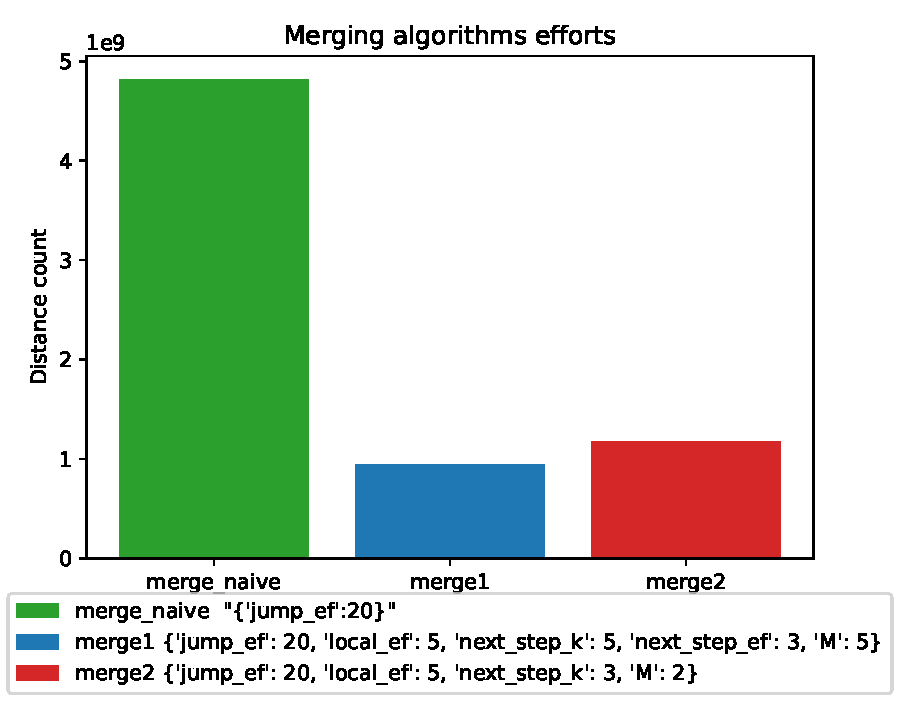
\includegraphics[width=1.\linewidth]{figs/merge-effort-comparison.pdf}
  \caption{Merging efforts}
  \label{fig:sfig1}
\end{subfigure}%
\begin{subfigure}{.5\textwidth}
  \centering
  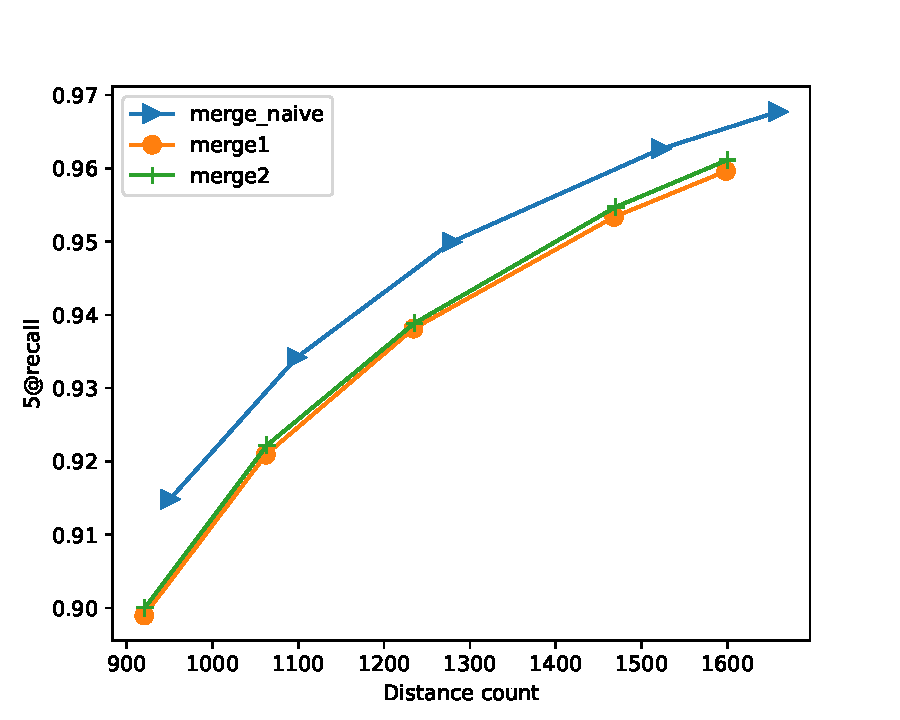
\includegraphics[width=1.\linewidth]{figs/recall-comparsion.pdf}
  \caption{Recall/computation trade off}
  \label{fig:sfig2}
\end{subfigure}
\caption{Merging algorithm comparison}
\label{fig:fig}
\end{figure}




\bibliographystyle{plain}
\bibliography{references}
\end{document}
